\documentclass[11pt]{article}
\usepackage[paperwidth=172mm,paperheight=243mm,left=18mm,right=18mm,top=20mm,bottom=20mm]{geometry}
\usepackage[T1]{fontenc}
\usepackage{lmodern,microtype,amsmath,amssymb,amsthm,mathtools,enumitem,graphicx,xcolor,hyperref,fancyhdr,booktabs}
\usepackage{float}
\hypersetup{colorlinks=true,linkcolor=blue!45!black,urlcolor=blue!45!black}
\graphicspath{{../figures/}}
\setlength{\parindent}{0pt}
\setlength{\parskip}{0.6em}
\setlist[enumerate]{itemsep=.25em,topsep=.2em}
\setlist[itemize]{itemsep=.2em,topsep=.2em}
\renewcommand{\baselinestretch}{1.045}
\pagestyle{fancy}\fancyhf{}\fancyhead[L]{\footnotesize INFORMATION GEOMETRY FOR THE IMPATIENT}\fancyhead[R]{\footnotesize THE MATHEMATICAL CORE}\fancyfoot[C]{\thepage}\renewcommand{\headrulewidth}{0.3pt}
\newtheorem{theorem}{Theorem}[section]
\newtheorem{proposition}[theorem]{Proposition}
\newtheorem{lemma}[theorem]{Lemma}
\newtheorem{corollary}[theorem]{Corollary}
\theoremstyle{definition}\newtheorem{definition}[theorem]{Definition}\newtheorem{exercise}{Problem}[section]
\newcommand{\D}{\mathcal D}\newcommand{\Pp}{\mathcal P}
\newcommand{\EE}{\mathbb E}\newcommand{\RR}{\mathbb R}
\newcommand{\ip}[2]{\langle #1,#2\rangle}
\newcommand{\KL}{\mathrm{KL}}
\newcommand{\grad}{\nabla}
\setcounter{section}{6}\setcounter{page}{23}
\begin{document}
\begin{center}
{\Large\bfseries Part II --- The Mathematical Core}\par
\vspace{.3em}
{\small Research extension for Working Edition 0.2 --- November 2026}\par
\end{center}

This extension is intended to be read immediately after the original four-chapter mathematical narrative and ten solved exercises. It strengthens the central claims rather than replacing the original pedagogical examples. In particular, we pass from the statement that Fisher geometry is ``natural'' to a finite, precise uniqueness theorem, with the invariance hypothesis exposed and the proof written out. Subsequently, divergence, duality, projection and natural-gradient flow become the consequences of stated formulas rather than metaphors.

\textbf{Notational agreement.} A simplex with $n$ outcomes has dimension $n-1$; all our probability coordinates are strictly positive unless explicitly stated. For a stochastic matrix $K$, the \emph{columns} sum to one and $q=Kp$. We use KL in the directional order $\KL(p\Vert q)$; reversing its arguments changes the induced affine orientation. In the original edition's Gaussian example, the straight mixture path means \emph{affine in expectation coordinates}; the literal mixture of two Gaussian densities usually is not Gaussian.

\section{Why Fisher geometry is forced}

\subsection{The mathematical problem}

Let
\[
 \Pp_n^\circ=\bigl\{p=(p_1,\ldots,p_n):p_i>0,\quad\sum_i p_i=1\bigr\},
 \qquad T_p\Pp_n^\circ=\{u\in\RR^n:\sum_i u_i=0\}.
\]
A Riemannian metric is a smoothly $p$-dependent positive-definite inner product $g^{(n)}_p(u,v)$ on each tangent space. There are infinitely many: besides the Fisher metric one can restrict the ordinary Euclidean metric $\sum_i u_iv_i$ to the simplex. Both transform tensorially when one changes coordinates. Therefore \emph{reparameterization invariance alone cannot possibly select Fisher geometry}.

We need an invariance principle involving the \emph{statistical experiment}, not merely the way its parameters are labelled. An experiment in which a symbol is randomly relabelled or split into several perfectly decodable symbols has not become more informative about $p$. Geometry should reflect that fact.

\begin{definition}[Stochastic channel and congruent embedding]
A stochastic channel from an $n$-outcome experiment to an $m$-outcome experiment is a matrix $K\in\RR^{m\times n}$ with $K_{ai}\ge0$ and $\sum_a K_{ai}=1$ for every input $i$. It maps $p\mapsto Kp$ and tangent vectors $u\mapsto Ku$. A channel $K$ is a \emph{congruent embedding} if there exists a stochastic recovery map $L$ with $LK=I_n$. Equivalently, its input columns have disjoint output supports (after removing output symbols never seen).
\end{definition}

A congruent embedding may add irrelevant random detail to each symbol, but the original symbol is recoverable without error. Example: the outcome $i$ may be split into $a_i$ children, each conditionally equiprobable. Its child probabilities are $p_i/a_i$. The recovery map merely forgets which child was seen.

\begin{theorem}[Finite-simplex \v{C}encov uniqueness; precisely scoped]\label{thm:chentsov}
For each integer $n\ge2$, let $g^{(n)}$ be a continuous Riemannian metric on $\Pp_n^\circ$. Suppose that for every congruent stochastic embedding $K:\Pp_n^\circ\to\Pp_m^\circ$, including coordinate permutations, we have
\[
 g^{(n)}_p(u,v)=g^{(m)}_{Kp}(Ku,Kv).
\]
Then there is a single constant $c>0$, independent of $n$, such that
\begin{equation}\label{eq:fisher-unique}
 \boxed{\quad g^{(n)}_p(u,v)=c\sum_{i=1}^n\frac{u_iv_i}{p_i}.\quad}
\end{equation}
Conversely, this family of Fisher metrics satisfies congruent-embedding invariance.
\end{theorem}

The theorem concerns a compatible \emph{family across all finite simplexes}. It makes no claim that merely choosing a coordinate-invariant metric on one isolated statistical model selects Fisher, and does not assert uniqueness among all monotone quantum metrics. We now prove it rather than appeal to authority.

\subsection{Proof: symmetry, common refinements and rational points}

\begin{proof}[Proof of Theorem~\ref{thm:chentsov}]
\textbf{Step 1: uniform barycentres.} Write $b_n=(1/n,\ldots,1/n)$. Every coordinate permutation fixes $b_n$. Its action on the tangent hyperplane $\sum_i u_i=0$ is the standard permutation representation. A permutation-invariant symmetric bilinear form on this hyperplane must be a scalar multiple of the restriction of the Euclidean inner product. Indeed, a permutation-invariant symmetric matrix on $\RR^n$ has constant diagonal and constant off-diagonal entries, hence the form $aI+b\mathbf{1}\mathbf{1}^{\!T}$, whose second term vanishes on the tangent hyperplane. Thus for some $C_n>0$,
\begin{equation}\label{eq:uniform}
  g^{(n)}_{b_n}(u,v)=C_n\sum_{i=1}^n u_iv_i.
\end{equation}

\textbf{Step 2: uniform refinements synchronize all dimensions.} For every integer $k\ge1$, split \emph{each} of the $n$ symbols into $k$ equally likely children. The embedding $K_{n,k}$ maps $b_n\mapsto b_{nk}$ and replaces $u_i$ by $k$ copies of $u_i/k$. Invariance and (\ref{eq:uniform}) give
\[
 C_n\sum_i u_iv_i=C_{nk}\sum_{i=1}^n\sum_{r=1}^k\frac{u_iv_i}{k^2}
 =\frac{C_{nk}}{k}\sum_i u_iv_i.
\]
Therefore $C_{nk}=kC_n$. Applying the same argument to $m$ and $n$ using their common multiple $mn$ yields $mC_n=nC_m$. Consequently $C_n/n=c$ is one and the same positive constant for every $n$.

\textbf{Step 3: rational distributions reduce to uniform ones.} Suppose $p_i=a_i/N$ where each $a_i$ is a positive integer and $N=\sum_i a_i$. Split symbol $i$ into $a_i$ equiprobable children. The resulting distribution is $b_N$, while $u_i$ becomes $a_i$ copies of $u_i/a_i$. By invariance,
\[
 g^{(n)}_p(u,v)=g^{(N)}_{b_N}(Ku,Kv)
 =C_N\sum_i a_i\frac{u_i}{a_i}\frac{v_i}{a_i}
 =cN\sum_i\frac{u_iv_i}{a_i}=c\sum_i\frac{u_iv_i}{p_i}.
\]
Strictly positive rational distributions are dense in $\Pp_n^\circ$. Both sides depend continuously on $p$ at every interior point, so (\ref{eq:fisher-unique}) follows for all interior $p$ and fixed tangent $u,v$.

\textbf{Converse.} For a congruent embedding, let $J_i$ be the disjoint output block arising from input $i$. For output $a\in J_i$ we have $(Kp)_a=K_{ai}p_i$, $(Ku)_a=K_{ai}u_i$, and similarly for $v$. Hence
\[
\sum_{a}\frac{(Ku)_a(Kv)_a}{(Kp)_a}
 =\sum_i\sum_{a\in J_i}K_{ai}\frac{u_iv_i}{p_i}
 =\sum_i\frac{u_iv_i}{p_i}.
\]
This proves the required invariance.\qedhere
\end{proof}

\paragraph{What did the proof actually use?} Only three ideas: permutation symmetry at the uniform distribution, invariance under splitting outcomes into decodable sub-outcomes, and continuity. The argument is deliberately restricted to finite positive probability vectors and a compatible system of metrics. It should not be extrapolated carelessly to singular models, infinite-dimensional families or quantum state spaces.

\subsection{A test that ordinary Euclidean geometry fails}

For a Bernoulli experiment $p=(1/2,1/2)$ and tangent $u=(t,-t)$, the metric induced by the ambient Euclidean norm gives $g^E_p(u,u)=2t^2$. If we split both outcomes into two equiprobable children, then $Ku=(t/2,t/2,-t/2,-t/2)$ and $g^E_{Kp}(Ku,Ku)=t^2$. The statistical experiment has gained no information, yet its Euclidean squared length has changed by a factor of two. Fisher gives $4t^2$ before and after. Coordinate invariance is cheap; invariance under sufficient representations is a substantive demand.

\section{Data processing is geometry}\label{sec:processing}

\subsection{Why noisy channels contract the Fisher metric}

The uniqueness theorem spoke only of information-preserving embeddings. General stochastic channels \emph{discard} information. The corresponding metric inequality is an infinitesimal data-processing principle.

\begin{proposition}[Fisher contraction under a Markov channel]\label{prop:contraction}
Let $p\in\Pp_n^\circ$ and $u\in T_p\Pp_n^\circ$. Let $K$ be any finite stochastic channel for which $q=Kp$ has strictly positive output coordinates. Then
\begin{equation}\label{eq:contraction}
 \sum_a\frac{(Ku)_a^2}{(Kp)_a}\ \leq\ \sum_i\frac{u_i^2}{p_i}.
\end{equation}
Equality holds precisely when the score $u_i/p_i$ is recoverable as a function of the observed output $Y$ almost surely under the joint law $\Pr(X=i,Y=a)=p_iK_{ai}$.
\end{proposition}

\begin{proof}
Define the score random variable $S(X)=u_X/p_X$. Since $q_a=\sum_i p_iK_{ai}$,
\[
 \EE[S(X)\mid Y=a]=\frac{\sum_i K_{ai}u_i}{\sum_i K_{ai}p_i}
 =\frac{(Ku)_a}{q_a}.
\]
Conditional Jensen's inequality gives $\EE[\EE(S\mid Y)^2]\le\EE[S^2]$. Those two expectations are exactly the left and right sides of (\ref{eq:contraction}). The equality condition is the equality case for the orthogonal projection in $L^2$: $S=\EE(S\mid Y)$ almost surely.\qedhere
\end{proof}

This proof is also a useful conceptual bridge: information geometry measures the variance of the score, and a stochastic channel replaces the score by its conditional expectation. In the terminology of statistical decision theory, the channel cannot manufacture local distinguishability.

\begin{corollary}[Local consequence of KL data processing]
For nearby positive laws $p$ and $p+\varepsilon u$, 
\[
 \KL(p\Vert p+\varepsilon u)=\frac{\varepsilon^2}{2}\sum_i\frac{u_i^2}{p_i}+O(\varepsilon^3).
\]
The usual data-processing inequality $\KL(Kp\Vert Kq)\le\KL(p\Vert q)$ therefore yields (\ref{eq:contraction}) by comparison of quadratic terms; Proposition~\ref{prop:contraction} additionally identifies the equality condition directly.
\end{corollary}

\begin{figure}[ht]
\centering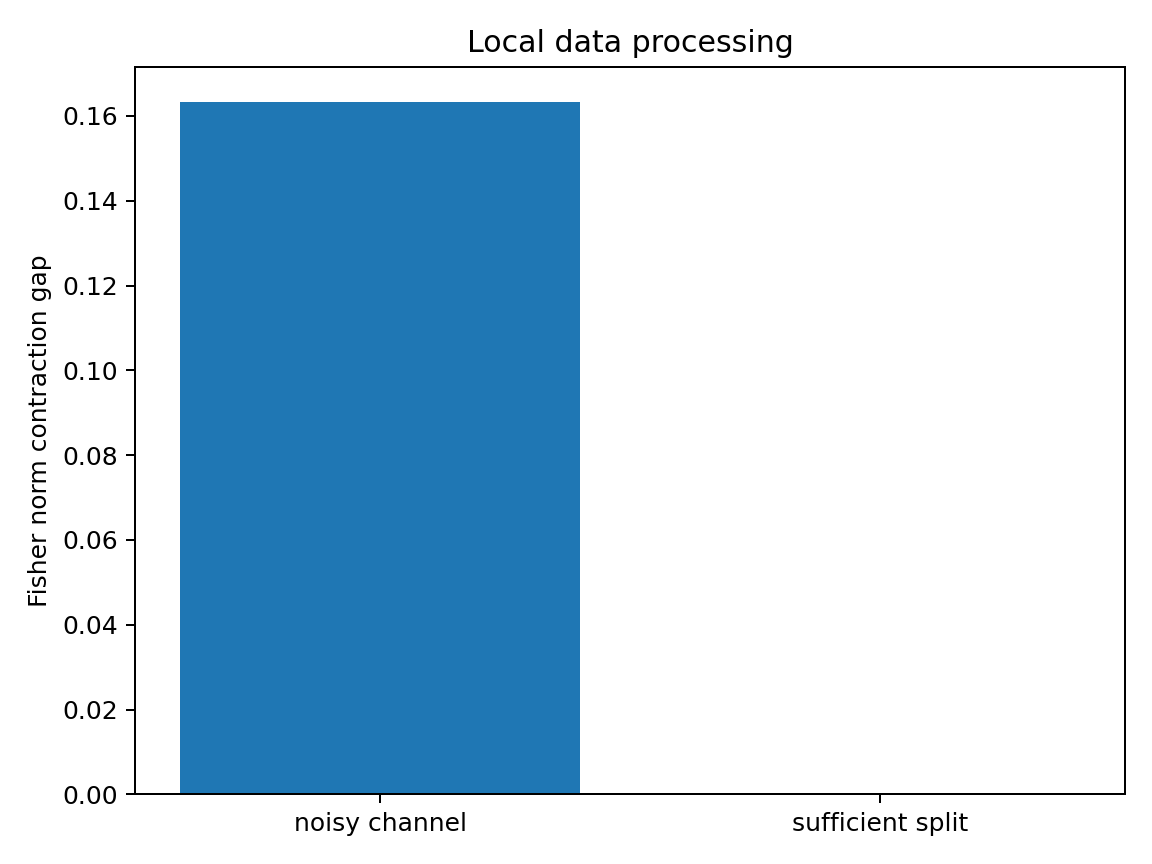
\includegraphics[width=.81\linewidth]{data_processing.png}
\caption{A noisy channel strictly contracts the Fisher squared norm of a chosen tangent vector; a sufficient refinement preserves it. The values are generated and verified by IG-Lab.}
\end{figure}

\subsection{The boundary warning that matters}

Do not infer from the Gaussian example that \emph{every} statistical boundary is infinitely distant. The square-root embedding of the categorical simplex into a sphere of radius two gives the boundary finite intrinsic distance. A Bernoulli probability $p\to0$ lies at finite Fisher distance from $p=1/2$, namely $\pi/2$. On the other hand, along the Gaussian variance ray $\sigma\to0$ with fixed mean, the length $\sqrt{2}\int d\sigma/\sigma$ diverges. These boundary behaviours differ because they belong to different statistical manifolds. In either case, singular boundary points are not ordinary positive interior models.

\section{A divergence creates more than a metric}\label{sec:divergence}

\subsection{Metric and affine connections from derivatives}

A smooth contrast $D(\theta,\theta')$ has $D\ge0$ and $D(\theta,\theta)=0$. Assuming suitable regularity and nondegeneracy, its mixed Hessian on the diagonal defines
\begin{equation}\label{eq:eguchi-g}
 g_{ij}(\theta)=-\left.\partial_i\partial_{j'}D(\theta,\theta')\right|_{\theta'=\theta}.
\end{equation}
The first derivatives vanish along the diagonal, but the third derivatives need not. Two torsion-free affine connections arise, in lowered-index form, as
\begin{align}\label{eq:eguchi-gammas}
\Gamma_{ij,k}&=-\left.\partial_i\partial_j\partial_{k'}D\right|_{\mathrm{diag}},\\
\Gamma^*_{ij,k}&=-\left.\partial_{i'}\partial_{j'}\partial_kD\right|_{\mathrm{diag}}.
\end{align}
Here a prime distinguishes derivatives in the second argument, and $\Gamma_{ij,k}=g_{k\ell}\Gamma^\ell_{ij}$. These symbols are not tensors individually, so one must not substitute a coordinate-free claim for the coordinate expressions. The two connections are \emph{dual} with respect to $g$:
\[
 Z[g(X,Y)]=g(\nabla_ZX,Y)+g(X,\nabla_Z^*Y).
\]
Their average is the Levi--Civita connection of $g$. Thus the second and third differential behaviour of a divergence contains information that the metric alone cannot encode.

\subsection{Exponential families and Legendre geometry}

Take a regular minimal exponential family on a common support,
\[
 p_\theta(x)=\exp\!\bigl(\theta\cdot T(x)-A(\theta)\bigr)h(x),
 \qquad \eta=\nabla A(\theta)=\EE_\theta[T(X)].
\]
Strict convexity of $A$ on its regular natural parameter domain implies
\[
 g_{ij}(\theta)=\partial_i\partial_j A(\theta),\qquad
 A^*(\eta)=\theta\cdot\eta-A(\theta),\quad \nabla A^*(\eta)=\theta.
\]
The KL divergence between two points of the family is exactly
\begin{equation}\label{eq:KL-Bregman}
 \KL(p_\theta\Vert p_{\theta'})
 =A(\theta')-A(\theta)-\eta(\theta)\cdot(\theta'-\theta)
 =B_A(\theta',\theta)=B_{A^*}(\eta,\eta'),
\end{equation}
where $B_F(x,y):=F(x)-F(y)-\nabla F(y)\cdot(x-y)$. Observe the argument order: with the convention (\ref{eq:KL-Bregman}), KL is \emph{reversed} Bregman divergence in natural coordinates.

One can now derive the affine connections explicitly. Insert $D(\theta,\theta')=B_A(\theta',\theta)$ into (\ref{eq:eguchi-g})--(\ref{eq:eguchi-gammas}); straightforward differentiation yields
\begin{equation}\label{eq:dualflatforms}
 g_{ij}=A_{ij},\qquad \Gamma_{ij,k}=A_{ijk},\qquad \Gamma^*_{ij,k}=0.
\end{equation}
Under \emph{this} orientation of $D$, the starred connection is exponential-flat in natural $\theta$ coordinates, while the unstarred connection is mixture-flat in dual $\eta$ coordinates. Reversing the arguments of the divergence interchanges them. The fundamental duality relation reduces to $\partial_k g_{ij}=A_{ijk}$.

\subsection{A third-order tensor, not a slogan}

The score's third moment, the Amari--Chentsov cubic tensor,
\[
 T_{ijk}=\EE_\theta[\partial_i\log p_\theta\,\partial_j\log p_\theta\,\partial_k\log p_\theta],
\]
is a genuine symmetric $(0,3)$ tensor. For an exponential family, $T_{ijk}=A_{ijk}$ in natural coordinates. Formula (\ref{eq:dualflatforms}) can therefore be summarized as a relationship between the exponential, mixture and Levi--Civita connections. In natural coordinates the latter has lowered coefficients $\tfrac12 A_{ijk}$. The affine connections are flat even when the metric curvature is nonzero: their curvature tensors are different mathematical objects.

\subsection{Gaussian geometry as an exact warning against conflation}

For a univariate Gaussian, let
\[
\theta_1=\frac{\mu}{\sigma^2},\quad \theta_2=-\frac1{2\sigma^2},\qquad
\eta_1=\mu,\quad\eta_2=\mu^2+\sigma^2.
\]
Linear interpolation in $\theta$ gives the exponential-affine path; linear interpolation in $\eta$ gives the mixture-affine path inside the Gaussian family. For endpoints $N(-a,1)$ and $N(a,1)$ the midpoint means vanish, while the midpoint \emph{variances} are
\[
 \sigma_{e}^2=1,\qquad \sigma_{m}^2=1+a^2,\qquad
 \sigma_{\mathrm{FR}}^2=1+\frac{a^2}{2}.
\]
The last formula follows from the Fisher isometry to $2(du^2+dv^2)/v^2$ with $u=\mu$ and $v=\sqrt2\sigma$: the Fisher geodesic is a semicircle orthogonal to the boundary. Its constant negative curvature is $-1/2$. None of these facts contradicts dual flatness.

\begin{figure}[ht]
\centering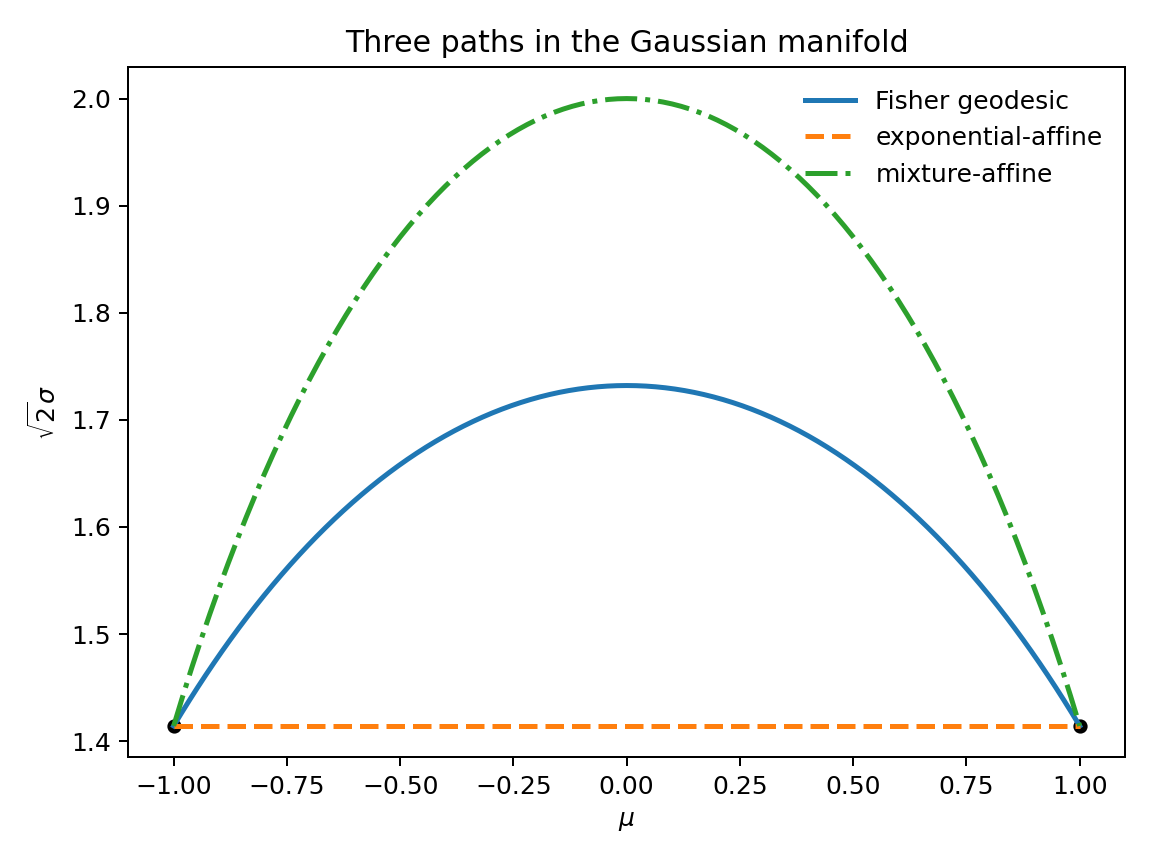
\includegraphics[width=.89\linewidth]{gaussian_three_paths.png}
\caption{The three Gaussian paths genuinely differ. The vertical axis is $v=\sqrt2\sigma$. In general, the plotted parameter of the circular path is Euclidean angle rather than Fisher arc length.}
\end{figure}

\section{Projection, orthogonality and Pythagoras}\label{sec:projection}

\subsection{The identity behind the theorem}

For differentiable strictly convex $F$ on a convex domain, the Bregman three-point identity is
\begin{equation}\label{eq:threepoint}
 B_F(x,z)=B_F(x,y)+B_F(y,z)
 +\ip{x-y}{\nabla F(y)-\nabla F(z)}.
\end{equation}
To prove it, write the definition of all three Bregman terms and cancel the three values of $F$. There is nothing approximate in this identity. It also warns us against the misleading slogan that every KL projection automatically satisfies an equality of squared distances.

\begin{theorem}[Pythagorean inequality and affine equality]\label{thm:pythag}
Let $C$ be a convex subset of the domain of differentiable strictly convex $F$; assume a minimizer $y\in C$ of $B_F(x,z)$ over $x\in C$ exists. Then for every $x\in C$,
\begin{equation}\label{eq:pythag}
 B_F(x,z)\ge B_F(x,y)+B_F(y,z).
\end{equation}
If $C$ is an affine slice and $y$ lies in its relative interior, the inequality is an equality for every $x\in C$.
\end{theorem}

\begin{proof}
Differentiating the objective $x\mapsto B_F(x,z)$ at the minimizer $y$ gives the first-order convex optimality condition
$\ip{x-y}{\nabla F(y)-\nabla F(z)}\ge0$ for all $x\in C$. Insert it into (\ref{eq:threepoint}) to obtain (\ref{eq:pythag}). On an affine slice with an interior constrained optimum, both positive and negative sufficiently small feasible displacements are allowed; therefore the directional derivative vanishes along its tangent space, making the inner product zero for every $x-y$ in that space.\qedhere
\end{proof}

\subsection{A complete three-outcome example}

Fix $q=(q_1,q_2,q_3)$ in the positive three-simplex and constrain $p_1=p_2$. Consider the \emph{forward} KL projection
\[
 r=\operatorname*{argmin}_{p\in\Pp_3^\circ,\ p_1=p_2}\KL(p\Vert q).
\]
Writing $p=(a,a,1-2a)$, direct differentiation with respect to $a$ gives
\[
\log\frac{a^2}{q_1q_2}-2\log\frac{1-2a}{q_3}=0,
\qquad \frac{a}{1-2a}=\frac{\sqrt{q_1q_2}}{q_3}.
\]
Therefore, with $z=q_3+2\sqrt{q_1q_2}$,
\begin{equation}\label{eq:closedprojection}
 \boxed{\quad r=\left(\frac{\sqrt{q_1q_2}}z,\frac{\sqrt{q_1q_2}}z,\frac{q_3}z\right).\quad}
\end{equation}
The affine constraint is a line in mixture coordinates, and $r$ lies in its interior. The exact Pythagorean equality becomes
\[
 \KL(p\Vert q)=\KL(p\Vert r)+\KL(r\Vert q),\qquad p_1=p_2.
\]
For $q=(0.6,0.3,0.1)$, the projection is approximately
\[ (0.447287,\ 0.447287,\ 0.105427). \]
IG-Lab checks the closed formula, first-order optimality and Pythagorean identity independently. Notice that minimizing $\KL(q\Vert p)$ would be a different optimization problem with a different minimizer; orientation matters.

\section{Learning as a geometric dynamical system}\label{sec:learning}

\subsection{Why a natural gradient is mathematically forced}

On a statistical manifold equipped with metric matrix $G(\theta)$, the derivative $dL_\theta$ is a covector. The ordinary vector of partial derivatives depends on a choice of coordinates; it is \emph{not} the intrinsic direction of steepest descent. The Riemannian gradient is obtained by raising an index:
\begin{equation}\label{eq:grad}
 \bigl(\operatorname{grad}_g L\bigr)^i
 =\sum_jG^{ij}(\theta)\,\partial_jL.
\end{equation}
This follows directly from $g(\operatorname{grad}_gL,v)=dL(v)$ for every tangent $v$. Thus the negative natural-gradient flow is $\dot\theta=-G^{-1}\nabla L$ wherever $G$ is nonsingular.

The same direction follows from a local KL trust-region problem. Using the quadratic approximation
\[
\KL(p_\theta\Vert p_{\theta+\delta})=\tfrac12\delta^TG\delta+o(\|\delta\|^2),
\]
minimize the first-order loss change $\nabla L\cdot\delta$ subject to $\tfrac12\delta^TG\delta\le\varepsilon$. A Lagrange multiplier gives the direction $-G^{-1}\nabla L$ and the length-normalized step (when $\nabla L\ne0$)
\begin{equation}\label{eq:trust}
\delta=-\sqrt{\frac{2\varepsilon}{\nabla L^TG^{-1}\nabla L}}\;G^{-1}\nabla L.
\end{equation}
This is a \emph{local} approximation to the KL constraint, not an exact global KL ball. Singular Fisher matrices require separate treatment, not a silent inverse.

\subsection{Bernoulli: one motion in two coordinate systems}

For a Bernoulli observation $y\in\{0,1\}$, let $L(p)=-y\log p-(1-y)\log(1-p)$. Then
\[
 L'(p)=\frac{p-y}{p(1-p)},\quad g_{pp}=\frac1{p(1-p)},\quad
 \boxed{\ \dot p=-g^{pp}L'(p)=y-p.\ }
\]
In the logit coordinate $\theta=\log(p/(1-p))$, we instead obtain $\partial_\theta L=p-y$ and $g_{\theta\theta}=p(1-p)$, so
\[
 \dot\theta=\frac{y-p}{p(1-p)},\qquad
 \dot p=\frac{dp}{d\theta}\dot\theta=p(1-p)\dot\theta=y-p.
\]
The two coordinate computations give the \emph{same probability flow}, with exact solution $p(t)=y+(p(0)-y)e^{-t}$. A naive Euclidean gradient flow in $p$ is not the transform of the naive Euclidean gradient flow in $\theta$.

\begin{figure}[ht]
\centering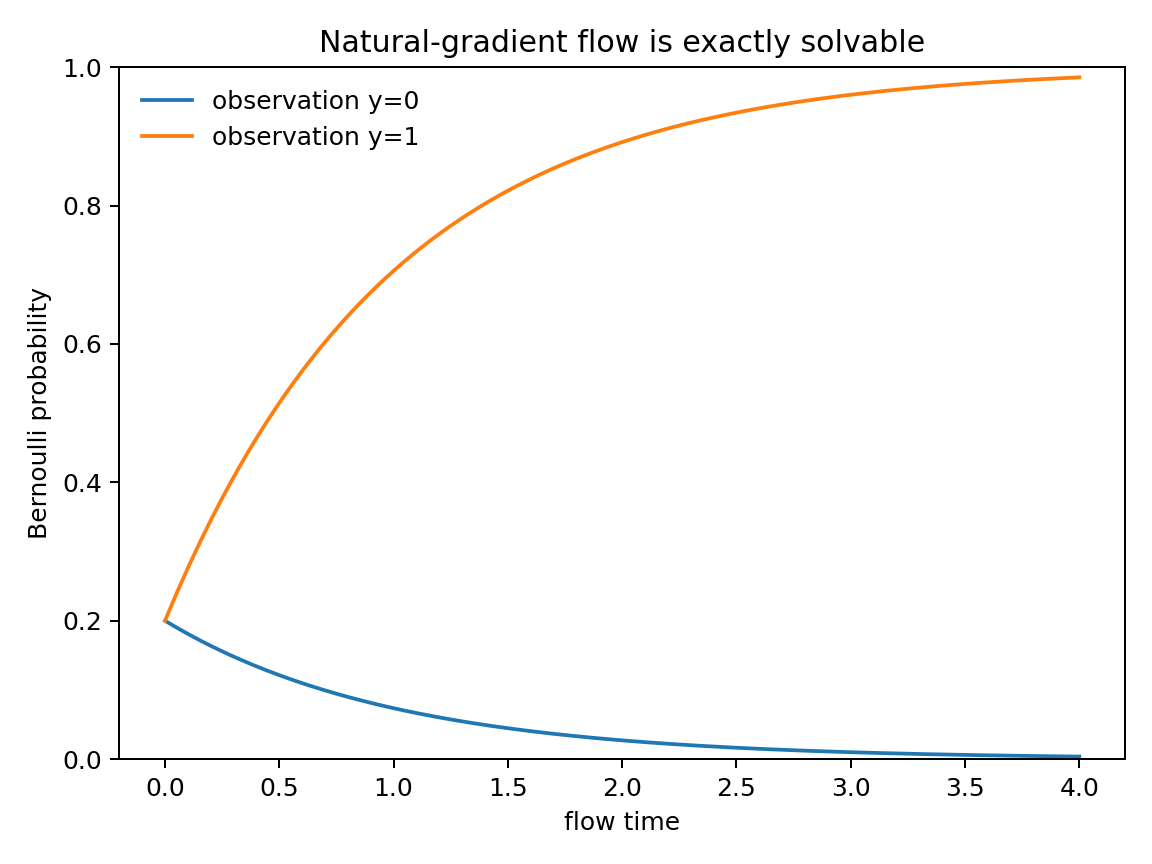
\includegraphics[width=.78\linewidth]{bernoulli_natural_flow.png}
\caption{Exact Bernoulli natural-gradient solutions, initialized at $p(0)=0.2$. For every finite $t$ and interior start, the flow remains strictly inside $(0,1)$.}
\end{figure}

\subsection{The replicator equation is a natural gradient}

Let $c=(c_1,\ldots,c_n)$ be a cost on outcomes and $L(p)=\sum_i p_i c_i$. On the simplex, the Fisher inner product is $g_p(u,v)=\sum_i u_iv_i/p_i$. The negative natural gradient of $L$, tangent to $\sum_i p_i=1$, is
\begin{equation}\label{eq:replicator}
 \boxed{\quad \dot p_i=-p_i\bigl(c_i-\overline{c}\bigr),\qquad
 \overline{c}=\sum_jp_jc_j.\quad}
\end{equation}
Indeed $\sum_i\dot p_i=0$ and for every tangent vector $v$,
\[
 g_p(\dot p,v)=-\sum_i(c_i-\overline c)v_i=-\sum_i c_iv_i=-dL_p(v).
\]
This proves the claim geometrically. It also gives a strict descent identity (unless all active costs coincide):
$\frac{d}{dt}L(p(t))=-\mathrm{Var}_{p(t)}(c)\le0$.
The dynamics preserve positivity for finite time when started inside the simplex.

\subsection{A boundary between two geometries: Fisher versus transport}

Information geometry is not the same as optimal transport. Fisher measures statistical distinguishability and depends only on the probabilities of the symbols; a Wasserstein metric additionally requires a \emph{ground distance} between outcomes. On the two-point space $\{0,1\}$ with ground distance one, write $p=(s,1-s)$ and $q=(t,1-t)$. The quadratic Wasserstein distance satisfies $W_2(p,q)^2=|s-t|$, whereas
\[
 d_{\mathrm{FR}}(p,q)=2\arccos\left(\sqrt{st}+\sqrt{(1-s)(1-t)}\right).
\]
Even in two dimensions these are different constructions. Their geodesics, infinitesimal structures and responses to coarse graining should not be conflated. Extending this comparison to continuous densities or unbalanced transport is a legitimate research direction, but not a missing lemma in \v{C}encov's theorem.

\section{Proof problems and computational checks}\label{sec:problems}

These problems are part of the mathematical argument, not padding. Each is paired with a concrete experiment or test in IG-Lab. The code can refute a proposed formula, but cannot prove a statement over all dimensions or real parameters.

\begin{exercise}[Uniqueness at uniform laws]
Prove that a bilinear form on $\sum_i u_i=0$ invariant under every coordinate permutation is a constant multiple of $\sum_i u_iv_i$. What changes if you demand invariance under only one transposition?
\end{exercise}
\emph{Check.} A matrix representing an invariant form must have equal diagonal and equal off-diagonal entries. One transposition leaves many other forms invariant when $n\ge3$; the full symmetric group is essential.

\begin{exercise}[A rational probability law]
Take $p=(2/10,3/10,5/10)$ and $u=(0.2,-0.1,-0.1)$. Construct a stochastic embedding into the uniform ten-outcome law, an explicit stochastic left inverse, and calculate the Fisher squared norm on both sides.
\end{exercise}
\emph{Answer.} Replicate coordinates in blocks of sizes $2,3,5$, giving child tangent values $(0.1,0.1;-1/30,-1/30,-1/30;-0.02,\ldots,-0.02)$. The squared Fisher norm is $0.2^2/0.2+0.1^2/0.3+0.1^2/0.5=0.253\overline3$ on both sides. The left inverse adds each block.

\begin{exercise}[The equality condition in data processing]
Show that $\EE[S\mid Y]$ has the same $L^2$ norm as $S$ if and only if $S$ is measurable with respect to $Y$. Explain why a sufficient refinement always gives equality, but a noisy channel may also give equality for \emph{some} tangent directions.
\end{exercise}
\emph{Answer.} Apply the orthogonal projection theorem: $\EE(S^2)=\EE(\EE(S\mid Y)^2)+\EE(\mathrm{Var}(S\mid Y))$. Zero conditional variance is the criterion. An individual score may be preserved even when other scores are lost.

\begin{exercise}[Do not reverse the KL convention]
For a regular exponential family, derive $\KL(p_\theta\Vert p_{\theta'})=B_A(\theta',\theta)$ directly from its logarithmic density. Check that the primed connection in natural coordinates has zero coefficients under the derivative convention (\ref{eq:eguchi-gammas}).
\end{exercise}
\emph{Answer.} Integrating $\log p_\theta-\log p_{\theta'}$ against $p_\theta$ gives $A(\theta')-A(\theta)-(\theta'-\theta)\cdot\eta(\theta)$. Differentiating it as prescribed gives $\Gamma^*_{ij,k}=0$, $\Gamma_{ij,k}=A_{ijk}$.

\begin{exercise}[Exact KL projection]
Derive (\ref{eq:closedprojection}) from one-variable calculus, then use the three-point identity to prove $\KL(p\Vert q)=\KL(p\Vert r)+\KL(r\Vert q)$ for any $p$ obeying $p_1=p_2$.
\end{exercise}
\emph{Answer.} The derivative of $\KL((a,a,1-2a)\Vert q)$ vanishes exactly when $a/(1-2a)=\sqrt{q_1q_2}/q_3$. Strict convexity ensures uniqueness; the affine tangent is orthogonal to $\nabla F(r)-\nabla F(q)$ for $F(p)=\sum p_i\log p_i$.

\begin{exercise}[Three midpoints, three answers]
Between $N(-a,1)$ and $N(a,1)$, calculate the exponential, mixture and Fisher midpoint variances. Show that for $a=2$ they are $1$, $5$, and $3$ respectively. Why is the literal mixture of the endpoint densities absent from this list?
\end{exercise}
\emph{Answer.} Natural coordinates keep precision fixed; expectation coordinates keep the second raw moment fixed; the Fisher semicircle has radius $\sqrt{a^2+2}$ in $(\mu,\sqrt2\sigma)$. The literal mixture density is bimodal for sufficiently separated means and is generally not a single Gaussian.

\begin{exercise}[Replicator flow]
Starting from $g_p(u,v)=\sum_i u_iv_i/p_i$, prove (\ref{eq:replicator}) for $L(p)=\sum_i p_ic_i$ and derive $\frac{dL}{dt}=-\mathrm{Var}_p(c)$. Explain why the projection onto the simplex tangent space contributes the mean-cost term.
\end{exercise}
\emph{Answer.} The Fisher dual of $dL$ can be represented by $p_ic_i$, but this has nonzero sum. Subtract $p_i\overline c$ to obtain a tangent vector. The descent derivative is $-\sum_i p_i(c_i-\overline c)c_i=-\mathrm{Var}_p(c)$.

\subsection{An explicit rigour ledger for the next edition}

\begin{tabular}{p{.25\linewidth}p{.64\linewidth}}
\toprule
\textbf{Claim} & \textbf{Scope and status}\\\midrule
Fisher uniqueness & Proved for compatible continuous metrics on all finite positive simplexes, invariant under congruent stochastic embeddings.\\
Data processing & Proved as score conditional-expectation contraction, with equality condition.\\
Dual flatness & Derived for regular minimal exponential families on common support; global complications at parameter-domain boundaries not included.\\
KL Pythagoras & Proved as convex projection inequality; equality only under appropriate affine/interiority hypotheses.\\
Natural gradient & Derived wherever the Fisher metric is nondegenerate; practical approximation and stochastic estimates need separate analysis.\\
Quantum/transport & Presented only as boundaries and future directions, not as theorems imported from the classical case.\\
\bottomrule
\end{tabular}

\subsection{Sources and further directions}

\begin{enumerate}
\item S. Amari and H. Nagaoka, \emph{Methods of Information Geometry}, AMS/Oxford, 2000. Foundations of dual connections and exponential families.
\item S. Amari, \emph{Information Geometry and Its Applications}, Springer, 2016. Especially the invariant metric on finite probability simplexes and congruent stochastic embeddings.
\item F. Nielsen, ``An Elementary Introduction to Information Geometry,'' \emph{Entropy} \textbf{22} (2020), 1100. Accessible companion on divergences and dualistic structures.
\item H. Nagaoka and S. Amari, ``Differential geometry of smooth families of probability distributions,'' \emph{Information Geometry} (2026).
\item S.-i. Amari, ``Differential geometry of curved exponential families---curvatures and information loss,'' \emph{Annals of Statistics} \textbf{10} (1982), 357--385.
\end{enumerate}

\end{document}
